\documentclass[slidestop]{beamer}
\usepackage{beamerthemesplit}
\usepackage{graphics}
\usepackage{pstricks}

\graphicspath{{./}}

\title{The Libre-SOC Hybrid 3D CPU}
\author{Luke Kenneth Casson Leighton}


\begin{document}

\frame{
   \begin{center}
    \huge{The Libre-SOC Hybrid 3D CPU}\\
    \vspace{32pt}
    \Large{Augmenting the OpenPOWER ISA}\\
    \Large{to provide 3D and Video instructions}\\
    \Large{(properly and officially)}\\
    \vspace{24pt}
    \Large{[proposed for] OpenPOWER Summit 2020}\\
    \vspace{16pt}
    \large{Sponsored by NLnet's PET Programme}\\
    \vspace{6pt}
    \large{\today}
  \end{center}
}


\frame{\frametitle{Why another SoC?}

\vspace{15pt}

 \begin{itemize}
   \item Intel Management Engine, QA issues, Spectre\vspace{15pt}
   \item Endless proprietary drivers \\
   		 (affects product development cost)\vspace{15pt}
   \item Opportunity to drastically simplify driver development\\
	     and engage in "long-tail" markets\vspace{15pt}
   \item Because for 30 years I Always Wanted To Design A CPU\vspace{10pt}
  \end{itemize}
}


\frame{\frametitle{Why OpenPOWER? (but first: Evaluation Criteria)}

\vspace{15pt}

 \begin{itemize}
   \item Good ecosystem essential\\
   		 linux kernel, u-boot, compilers, OSes,\\
   		 Reference Implementation(s)\vspace{12pt}
   \item Supportive Foundation and Members\\
   		 need to be able to submit ISA augmentations\\
   		 (for proper peer review)\vspace{12pt}
   \item No NDAs, full transparency must be acceptable\\
	     due to being funded under NLnet's PET Programme\vspace{12pt}
  \end{itemize}
}

\frame{\frametitle{Why OpenPOWER?}


 \begin{itemize}
   \item RISC-V: closed secretive mailing lists, closed secretive\\
   		 ISA Working Groups, no acceptance of transparency\\
   		 requirements, not well-established enough
   \item MIPS Open Initiative website was offline
   \item ARM and x86 are proprietary (x86 too complex)
   \item OpenRISC 1200 not enough adoption
   \item Nyuzi GPU too specialist (not a general-purpose ISA)
   \item MIAOW GPU is not a GPU (it's an AMD Vector Engine)
   \item "rolling your own" out of the question (20+ man-years)
   \item OpenPOWER: established for decades, excellent Foundation,\\
   	     Microwatt as Reference, approachable and friendly.
  \end{itemize}
}

\frame{\frametitle{What goes into a typical SoC?}
\vspace{9pt}
 \begin{itemize}
   \item 15 to 20mm BGA package: 2.5 to 5 watt power consumption\\
   		heat sink normally not required (simplifies overall design)
   		\vspace{10pt}
   \item Fully-integrated peripherals (not Northbridge/Southbridge)\\
         USB, HDMI, RGB/TTL, SD/MMC, I2C, UART, SPI, GPIO etc. etc. 
         \vspace{10pt}
   \item Built-in GPU (shared memory bus, 3rd party licensed) \vspace{10pt}
   \item Build-in VPU (likewise)\vspace{10pt}
   \item Target price between \$2.50 and \$30 depending on market\\
         Radically different from IBM POWER9 Core (200 Watt)
         \vspace{10pt}
  \end{itemize}
}



\frame{\frametitle{Simple SBC-style SoC}

\begin{center}
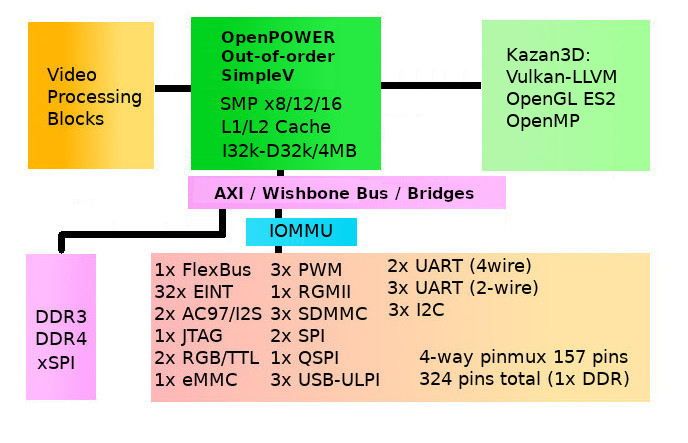
\includegraphics[width=0.9\textwidth]{shakti_libre_soc.jpg}
\end{center}

}


\frame{\frametitle{Where to start? (roadmap)}

 \begin{itemize}
   \item First thing: get a basic core working on an FPGA\\
         (use Microwatt as a reference)
   \item Next: create a low-cost test ASIC (180nm).\\
   		 (first OpenPOWER ASIC since IBM's POWER9, 10 years ago)
   \item (in parallel): Develop Vector ISA with 3D and Video\\
   		 extensions, under watchful eye of OpenPOWER Foundation
   \item Implement Vector ISA in simulator, then HDL, then FPGA\\
         and finally (only when ratified by OPF) into silicon
   \item Sell chips, make \$\$\$.
  \end{itemize}
}

\frame{\frametitle{What's different about Libre-SOC?}

 \begin{itemize}
   \item Hybrid - integrated.  The CPU \textit{is} the GPU.\\
         The GPU \textit{is} the CPU.  The VPU \textit{is} the CPU.\\
         \textit{There is No Separate VPU/GPU Pipeline}\\
   		  \vspace{9pt}
   \item written in nmigen (a python-based HDL).  Not VHDL\\
   		  not Verilog (definitely not Chisel3/Scala)\\
   		  This is an extremely important strategic decision.
   		  \vspace{9pt}
   \item Simple-V Vector Extension.  See "SIMD Considered harmful".\\
   		SV effectively a "hardware for-loop" on standard scalar ISA\\
   		(conceptually similar to Zero-Overhead Loops in DSPs)
   		  \vspace{9pt}
  \end{itemize}
}

\frame{\frametitle{Hybrid Architecture: Augmented 6600}

 \begin{itemize}
   \item CDC 6600 is a design from 1965.  The \textit{augmentations} are not.\\
   		 Help from Mitch Alsup includes \textit{precise exceptions}, \\
   		 multi-issue and more. Academic literature on 6600 utterly misleading.
   		6600 Scoreboards completely underestimated (Seymour Cray and
   		James Thornton
   		solved problems they didn't realise existed elsewhere!)
   \item Front-end Vector ISA, back-end "Predicated (masked) SIMD"\\
         nmigen (python OO) strategically critical to achieving this.
   \item Out-of-order combined with Simple-V allows scalar operations\\
         at the developer end to be turned into SIMD at the back-end\\
         \textit{without the developer needing to do SIMD}
   \item IEEE754 sin / cos / atan2, Texturisation opcodes, YUV2RGB\\
   		 all automatically vectorised.
  \end{itemize}
}

\frame{\frametitle{Why nmigen? (but first: evaluate other HDLs)}

 \begin{itemize}
   \item Verilog: designed in the 1980s purely for doing unit tests (!)
   \item VHDL: again, a 1980s-era "Procedural" language (BASIC, Fortran).
         Does now have "records" which is nice.
   \item Chisel3 / Scala: OO, but very obscure (20th on index)
   \item pyrtl: not large enough community
   \item MyHDL: subset of python only
         \vspace{9pt}
   \item Slowly forming a set of criteria: must be OO (python), must have
         wide adoption (python), must have good well-established
         programming practices already in place (python), must be
         easy to learn (python)
   \item HDL itself although a much smaller community must have the same
         criteria.  Only nmigen meets that criteria.
   
  \end{itemize}
}

\frame{\frametitle{Why nmigen?}

 \begin{itemize}
   \item Uses python to build an AST (Abstract Syntax Tree).
         Actually hands that over to yosys (to create ILANG file)
         after which verilog can (if necessary) be created
   \item Deterministic synthesiseable behaviour (Signals are declared
         with their reset pattern: no more forgetting "if rst" block).
   \item python OO programming techniques can be deployed.  classes
         and functions created which pass in parameters which change
         what HDL is created (IEEE754 FP16 / 32 / 64 for example)
   \item python-based for-loops can e.g. read CSV files then generate
         a hierarchical nested suite of HDL Switch / Case statements
         (this is how the Libre-soc PowerISA decoder is implemented)
   \item extreme OO abstraction can even be used to create "dynamic
         partitioned Signals" that have the same operator-overloaded
         "add", "subtract", "greater-than" operators
   
  \end{itemize}
}

\frame{\frametitle{nmigen (dynamic) vs VHDL (static)}

\begin{center}
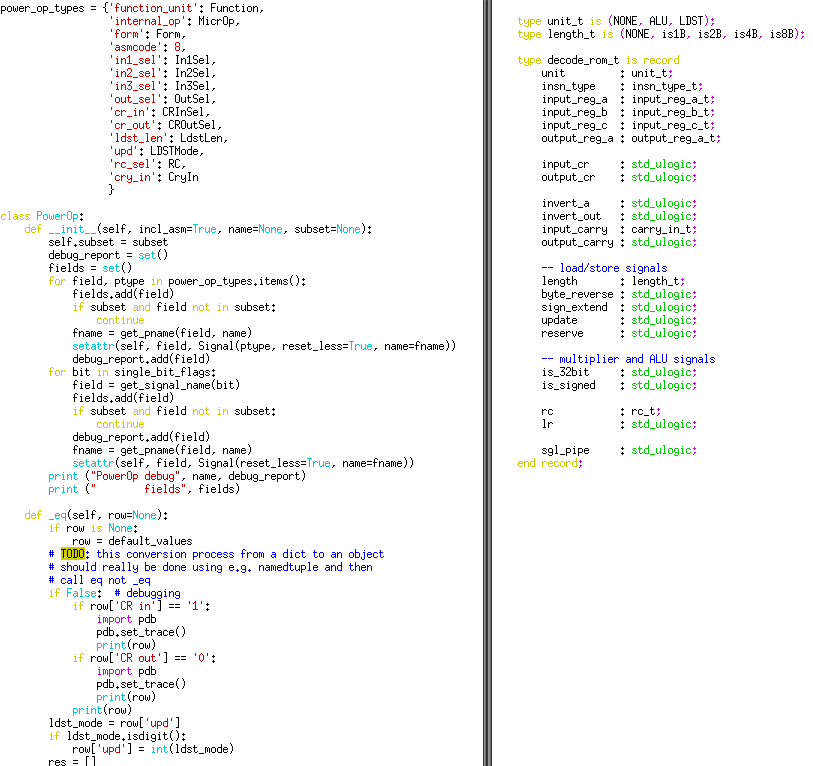
\includegraphics[width=1.0\textwidth]{2020-09-10_11-53.png}
\end{center}

}

\frame{\frametitle{nmigen PowerISA Decoder}

\begin{center}
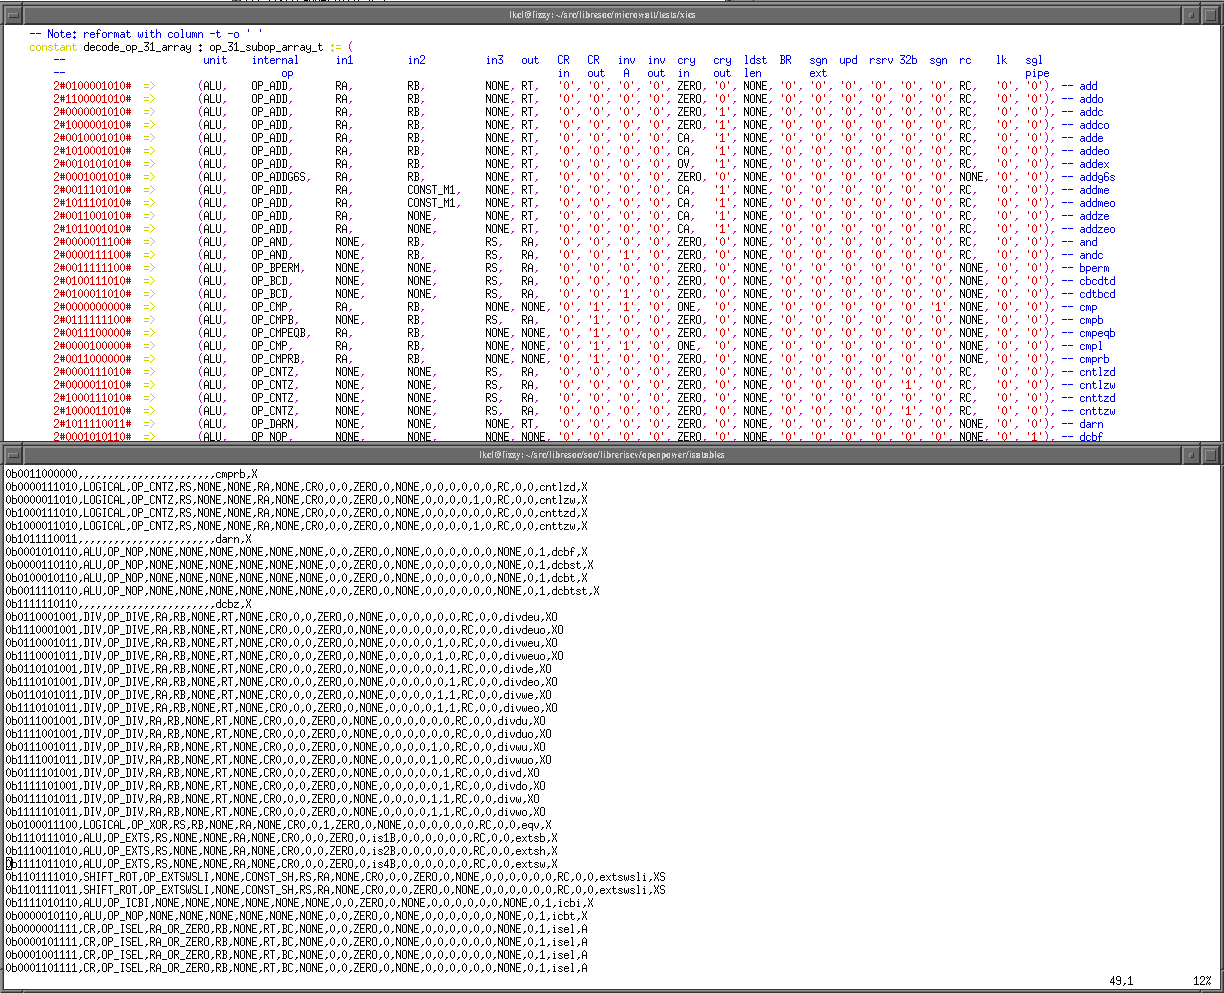
\includegraphics[width=1.0\textwidth]{2020-09-10_11-46.png}
\end{center}

}

\frame{\frametitle{nmigen PowerISA Decoder}

\begin{center}
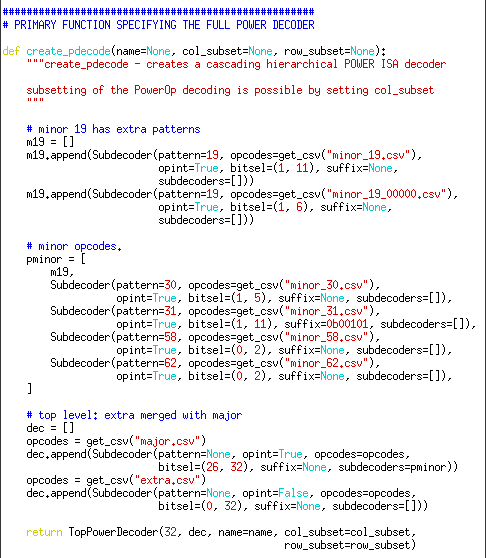
\includegraphics[width=0.55\textwidth]{2020-09-09_21-04.png}
\end{center}

}

\frame{\frametitle{Why another Vector ISA? (or: not-exactly another)}

 \begin{itemize}
   \item Simple-V is a 'register tag' system.  \textit{There are no opcodes}\\
   		 SV 'tags' scalar operations (scalar regfiles) as 'vectorised'
   \item (PowerISA SIMD is around 700 opcodes, making it unlikely to be
    	 able to fit a PowerISA decoder in only one clock cycle)
   \item Effectively a 'hardware sub-counter for-loop': pauses the PC\\
         then rolls incrementally through the operand register numbers\\
         issuing \textit{multiple} scalar instructions into the pipelines\\
         (hence the reason for a multi-issue OoO microarchitecture)
   \item Current \textit{and future} PowerISA scalar opcodes inherently
   	 	 \textit{and automatically} become 'vectorised' by SV without
   	 	 needing an explicit new Vector opcode.
   \item Predication and element width polymorphism are also 'tags'.
         elwidth polymorphism allows for FP16 / 80 / 128 to be added to
         the ISA \textit{without modifying the ISA}
   
  \end{itemize}
}


\begin{frame}[fragile]
\frametitle{Simple-V ADD in a nutshell}

\begin{semiverbatim}
function op\_add(rd, rs1, rs2, predr) # add not VADD!
  int i, id=0, irs1=0, irs2=0;
  for (i = 0; i < VL; i++)
    if (ireg[predr] & 1<<i) # predication uses intregs
       ireg[rd+id] <= ireg[rs1+irs1] + ireg[rs2+irs2];
    if (reg\_is\_vectorised[rd] )  \{ id += 1; \}
    if (reg\_is\_vectorised[rs1])  \{ irs1 += 1; \}
    if (reg\_is\_vectorised[rs2])  \{ irs2 += 1; \}
\end{semiverbatim}

  \begin{itemize}
   \item Above is oversimplified: Reg. indirection left out (for clarity).
   \item SIMD slightly more complex (case above is elwidth = default)
   \item Scalar-scalar and scalar-vector and vector-vector now all in one
   \item OoO may choose to push ADDs into instr. queue (v. busy!)
  \end{itemize}
\end{frame}


\frame{\frametitle{Summary}

 \begin{itemize}
   \item Goal is to create a mass-volume low-power embedded SoC suitable
         for use in netbooks, chromebooks, tablets, smartphones, IoT SBCs.
   \item No DRM. 'Trustable' (by the users, not by Media Moguls) design
         ethos as a \textit{business} objective: requires full transparency
         as well as Formal Correctness Proofs
   \item Collaboration with OpenPOWER Foundation and Members absolutely
         essential. No short-cuts.  Standards to be developed and ratified
         so that everyone benefits.
   \item Working on the back of huge stability of POWER ecosystem
   \item Combination of which is that Board Support Package is 100\%
         upstream, app and product development by customer is hugely
         simplified and much more attractive
         
  \end{itemize}
}


\frame{
  \begin{center}
    {\Huge The end\vspace{15pt}\\
		   Thank you\vspace{15pt}\\
		   Questions?\vspace{15pt}
	}
  \end{center}
  
  \begin{itemize}
	\item Discussion: Libre-SOC-dev mailing list
	\item Freenode IRC \#libre-soc
	\item http://libre-soc.org/
	\item http://nlnet.nl/PET
  \end{itemize}
}


\end{document}
